\documentclass[11pt]{article}

% ------------------------------------------------------------------
%  Packages (all available on Overleaf by default)
% ------------------------------------------------------------------
\usepackage[a4paper,margin=2.6cm]{geometry}
\usepackage[T1]{fontenc}
\usepackage{lmodern}
\usepackage{microtype}
\usepackage{amsmath,amssymb,amsthm}
\usepackage{graphicx}
\usepackage{booktabs}
\usepackage{tabularx}
\usepackage{xltabular}
\usepackage{enumitem}
\usepackage[dvipsnames]{xcolor}
\usepackage{tikz}
\usepackage[most]{tcolorbox}
\usepackage[hidelinks]{hyperref}
\usepackage{caption}
\captionsetup{font=small,labelfont=bf}
\usepackage{listings}
\lstset{basicstyle=\ttfamily\small,columns=fullflexible,breaklines=true,frame=single,framesep=4pt}

% ------------------------------------------------------------------
%  Theorem environments
% ------------------------------------------------------------------
\theoremstyle{plain}
\newtheorem{lemma}{Lemma}[section]
\newtheorem{theorem}[lemma]{Theorem}
\newtheorem{proposition}[lemma]{Proposition}
\newtheorem{corollary}[lemma]{Corollary}
\newtheorem{conjecture}[lemma]{Conjecture}
\newtheorem*{pappus}{Pappus's centroid theorem}
\theoremstyle{definition}
\newtheorem{definition}[lemma]{Definition}
\newtheorem{example}[lemma]{Example}
\theoremstyle{remark}
\newtheorem{remark}[lemma]{Remark}

\newtcolorbox{sidebox}[1]{colback=gray!4,colframe=gray!60,fonttitle=\bfseries,title={#1},breakable,left=6pt,right=6pt}

\newcommand{\R}{\mathbb{R}}
\newcommand{\vol}{\operatorname{vol}}
\newcommand{\dd}{\,\mathrm{d}}

% ------------------------------------------------------------------
\title{From a Bent Cylinder to Centroid Curves:\\ When Does Pappus Still Work?}
\author{Baran Akter}
\date{November 2026}

\begin{document}
\maketitle

\begin{abstract}
About 1700 years ago Pappus of Alexandria noticed that a doughnut has the same volume as the straight cylinder you would get by cutting it open and straightening it. We start from this observation, explain with nothing more than first-year calculus why it is true, and show one dimension up (in $\R^4$) that the same trick produces an extra term. We then turn to a modern version of the question, due to H.~Schmid (2025): if you slice a solid perpendicular to a \emph{curved} curve, when do the areas of the slices add up exactly to the volume? This happens when every slice is balanced on the curve, and such curves are called \emph{centroid curves}. Our contributions are: (1) a short proof that the slices are allowed to overlap; (2) a complete description of the centroid curves of an ellipsoid, including the surprise that in an egg whose long axis is $\sqrt2$ times its width, \emph{every parabola through the centre} is a centroid curve; (3) a global existence result for centrally symmetric convex bodies under one stated hypothesis; and (4) evidence, partly with a computer-assisted proof, that in a solid torus centroid curves can run into a ``fold'' and get stuck. Results that rest on computation rather than proof are marked as such, and a table at the end summarises the status of each result.
\end{abstract}

\begin{figure}[h]
\centering
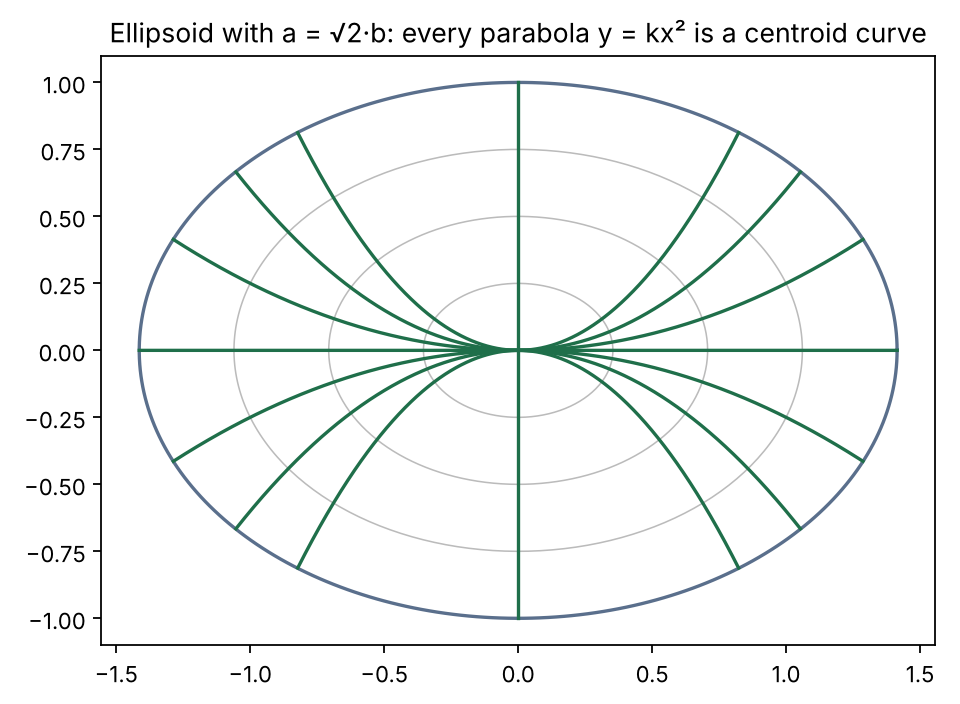
\includegraphics[width=0.47\textwidth]{figures/ellipsoid_parabolas.png}\hfill
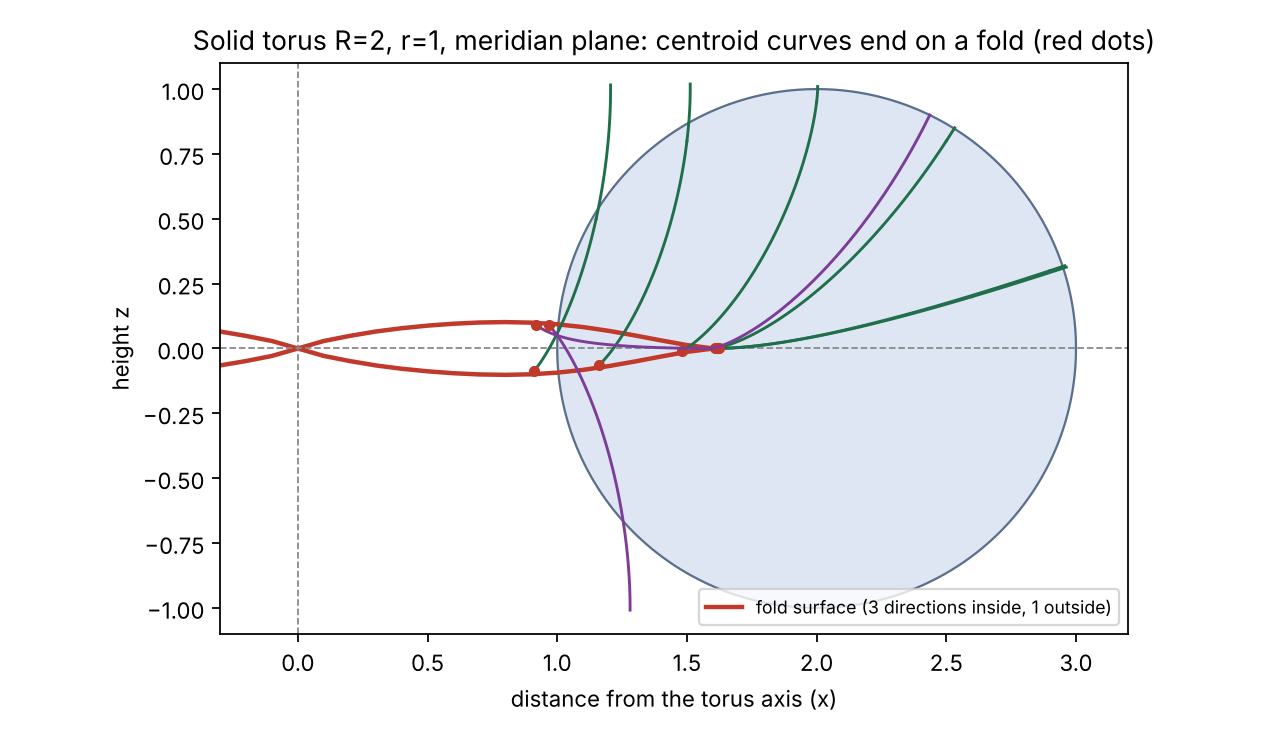
\includegraphics[width=0.51\textwidth]{figures/torus_meridian.png}
\caption{The two pictures this paper is about. \textbf{Left:} the middle cross-section of an ellipsoid whose axes satisfy $a=\sqrt2\,b$. Every green curve (every parabola $y=kx^2$, and the two axes) is a centroid curve: if you slice the egg perpendicular to it, the slices are balanced exactly on the curve and their areas add up to the volume (Section~\ref{sec:ellipsoid}). \textbf{Right:} a cross-section of a solid torus. The green and purple centroid curves start on the surface, run inwards, and end at red dots on a thin red ``fold'' where the direction they need stops existing (Section~\ref{sec:torus}).}
\label{fig:teaser}
\end{figure}

\tableofcontents

% ==================================================================
\section{1700 years ago: Pappus}\label{sec:history}
% ==================================================================

Pappus of Alexandria wrote his \emph{Collection} around the year 320~AD \cite{pappus}. In Book~VII, almost in passing, he states two rules for solids and surfaces made by spinning a flat shape around an axis. The rules were forgotten and rediscovered by the Swiss Jesuit Paul Guldin in the 1630s \cite{guldin}, which is why they are often called the Pappus--Guldin theorems. In modern language:

\begin{pappus}[\cite{pappus,guldin}]
Let $D$ be a region in a plane, and let $L$ be a line in the same plane that does not cut through $D$. Spin $D$ once around $L$. Then
\[
  \text{volume of the solid} \;=\; \text{area of } D \;\times\; \text{distance travelled by the centroid of } D .
\]
Likewise, the area of the surface swept by the boundary curve of $D$ equals the length of that curve times the distance travelled by the curve's own centroid.
\end{pappus}

The centroid is the ``balance point'' of the shape: the average of all its points. For a disc it is the centre. The first rule is the one we care about.

\begin{example}[The doughnut]\label{ex:torus}
Spin a disc of radius $r$ around a line at distance $R>r$ from its centre. The result is a solid torus (a doughnut). The centroid travels around a circle of length $2\pi R$, so
\[
  V_{\text{torus}} = \pi r^2 \cdot 2\pi R = 2\pi^2 R r^2 .
\]
The boundary circle has length $2\pi r$ and its centroid is also the centre, so the surface area is $2\pi r\cdot 2\pi R=4\pi^2Rr$.
\end{example}

Here is the observation that starts this paper. If you cut the doughnut once and straighten it, you get a cylinder of radius $r$ and length $2\pi R$. Its volume is $\pi r^2\cdot 2\pi R$, \emph{the same number}. So Pappus's rule says: \emph{bending a cylinder into a ring does not change its volume}. Why should that be true?

% ==================================================================
\section{The bent cylinder: why the doughnut works}\label{sec:cylinder}
% ==================================================================

\begin{figure}[h]
\centering
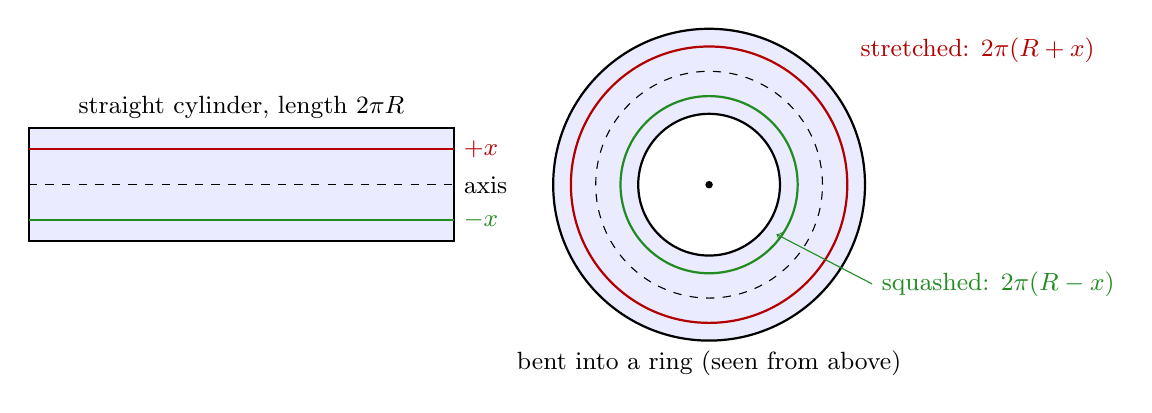
\begin{tikzpicture}[scale=0.9]
  % straight cylinder (side view)
  \fill[blue!8] (0,0) rectangle (6,1.6);
  \draw[thick] (0,0) rectangle (6,1.6);
  \draw[dashed] (0,0.8) -- (6,0.8);
  \draw[red!70!black,thick] (0,1.3) -- (6,1.3);
  \draw[ForestGreen,thick] (0,0.3) -- (6,0.3);
  \node[above] at (3,1.6) {\small straight cylinder, length $2\pi R$};
  \node[right,red!70!black] at (6,1.3) {\small $+x$};
  \node[right,ForestGreen] at (6,0.3) {\small $-x$};
  \node[right] at (6,0.8) {\small axis};
  % bent version (top view of the torus)
  \begin{scope}[xshift=9.6cm,yshift=0.8cm]
    \fill[blue!8,even odd rule] (0,0) circle (2.2) (0,0) circle (1.0);
    \draw[thick] (0,0) circle (2.2); \draw[thick] (0,0) circle (1.0);
    \draw[dashed] (0,0) circle (1.6);
    \draw[red!70!black,thick] (0,0) circle (1.95);
    \draw[ForestGreen,thick] (0,0) circle (1.25);
    \fill (0,0) circle (1.5pt);
    \node[below] at (0,-2.2) {\small bent into a ring (seen from above)};
    \node[red!70!black,right] at (2.0,1.9) {\small stretched: $2\pi(R+x)$};
    \node[ForestGreen,right] at (2.3,-1.4) {\small squashed: $2\pi(R-x)$}; \draw[ForestGreen,->] (2.3,-1.4) -- (0.95,-0.7);
  \end{scope}
\end{tikzpicture}
\caption{Bending a cylinder into a ring. A thread at distance $x$ outside the axis (red) is stretched to length $2\pi(R+x)$. Its mirror thread at distance $x$ inside (green) is squashed to $2\pi(R-x)$. Together they have length $4\pi R$, exactly as before bending.}
\label{fig:bend}
\end{figure}

Think of the cylinder as a bundle of thin straight threads, all of length $2\pi R$. When we bend it into a ring, a thread at horizontal distance $x$ \emph{outside} the axis ends up on a circle of radius $R+x$, so its length becomes $2\pi(R+x)$: it is stretched by the factor $1+x/R$. Its partner at distance $x$ \emph{inside} the axis ends up on a circle of radius $R-x$ and is squashed by $1-x/R$ (Figure~\ref{fig:bend}). The stretch and the squash cancel exactly:
\[
  2\pi(R+x) + 2\pi(R-x) = 2\cdot 2\pi R .
\]
Since the disc is symmetric, every thread has a partner, and the total volume does not change.

\subsection{The same argument as an integral}
Put coordinates $(x,y)$ in the disc $D$, with $x$ measured horizontally away from the axis of rotation. A small piece of area $\mathrm dA$ at $(x,y)$ sweeps out a thin ring of volume $2\pi(R+x)\,\mathrm dA$. Adding up,
\[
  V = \iint_D 2\pi(R+x)\dd A
    = 2\pi R\iint_D \mathrm dA \;+\; 2\pi\iint_D x\dd A
    = 2\pi R\cdot \pi r^2 + 0 .
\]
The second integral is zero because $x$ is measured from the centroid: positive and negative values cancel. \emph{That cancellation is the whole proof of Pappus's theorem.} For a general region $D$ the same computation gives $V=2\pi(R+\bar x)\cdot\operatorname{area}(D)$, where $\bar x$ is the centroid's offset, which is exactly the rule in Section~\ref{sec:history}.

\subsection{A check with cylindrical shells}
If you do not trust the argument, compute the volume a second way. Slice the disc into vertical strips at horizontal position $x\in[-r,r]$, each of height $2\sqrt{r^2-x^2}$. Each strip sweeps out a cylindrical shell of radius $R+x$:
\[
  V=\int_{-r}^{r}2\pi(R+x)\cdot 2\sqrt{r^2-x^2}\dd x
   = 4\pi R\underbrace{\int_{-r}^{r}\sqrt{r^2-x^2}\dd x}_{=\pi r^2/2}
   + 4\pi\underbrace{\int_{-r}^{r}x\sqrt{r^2-x^2}\dd x}_{=0\ (\text{odd})}
   = 2\pi^2Rr^2 .
\]

\begin{example}[An infinitely long solid with finite volume]\label{ex:gauss}
Let $D$ be the region under the bell curve, $0\le y\le e^{-x^2}$, and spin it around the horizontal line $y=-1$ (Figure~\ref{fig:gaussregion}). The region is infinitely long, but its area is $A=\int_{-\infty}^{\infty}e^{-x^2}\dd x=\sqrt\pi$. Its centroid height is
\[
  \bar y=\frac1A\int_{-\infty}^{\infty}\frac{\bigl(e^{-x^2}\bigr)^2}{2}\dd x=\frac{1}{2\sqrt\pi}\sqrt{\frac\pi2}=\frac{1}{2\sqrt2},
\]
so the centroid is at distance $R=1+\frac1{2\sqrt2}$ from the axis, and Pappus gives
\[
  V=\sqrt\pi\cdot 2\pi\Bigl(1+\tfrac1{2\sqrt2}\Bigr)=\pi^{3/2}\Bigl(2+\tfrac1{\sqrt2}\Bigr)\approx 15.07 .
\]
As a check, the washer method gives $V=\int_{-\infty}^{\infty}\pi\bigl[(1+e^{-x^2})^2-1\bigr]\dd x$, which a computer evaluates to the same value, $15.0740584801$.
\end{example}

\begin{figure}[h]
\centering
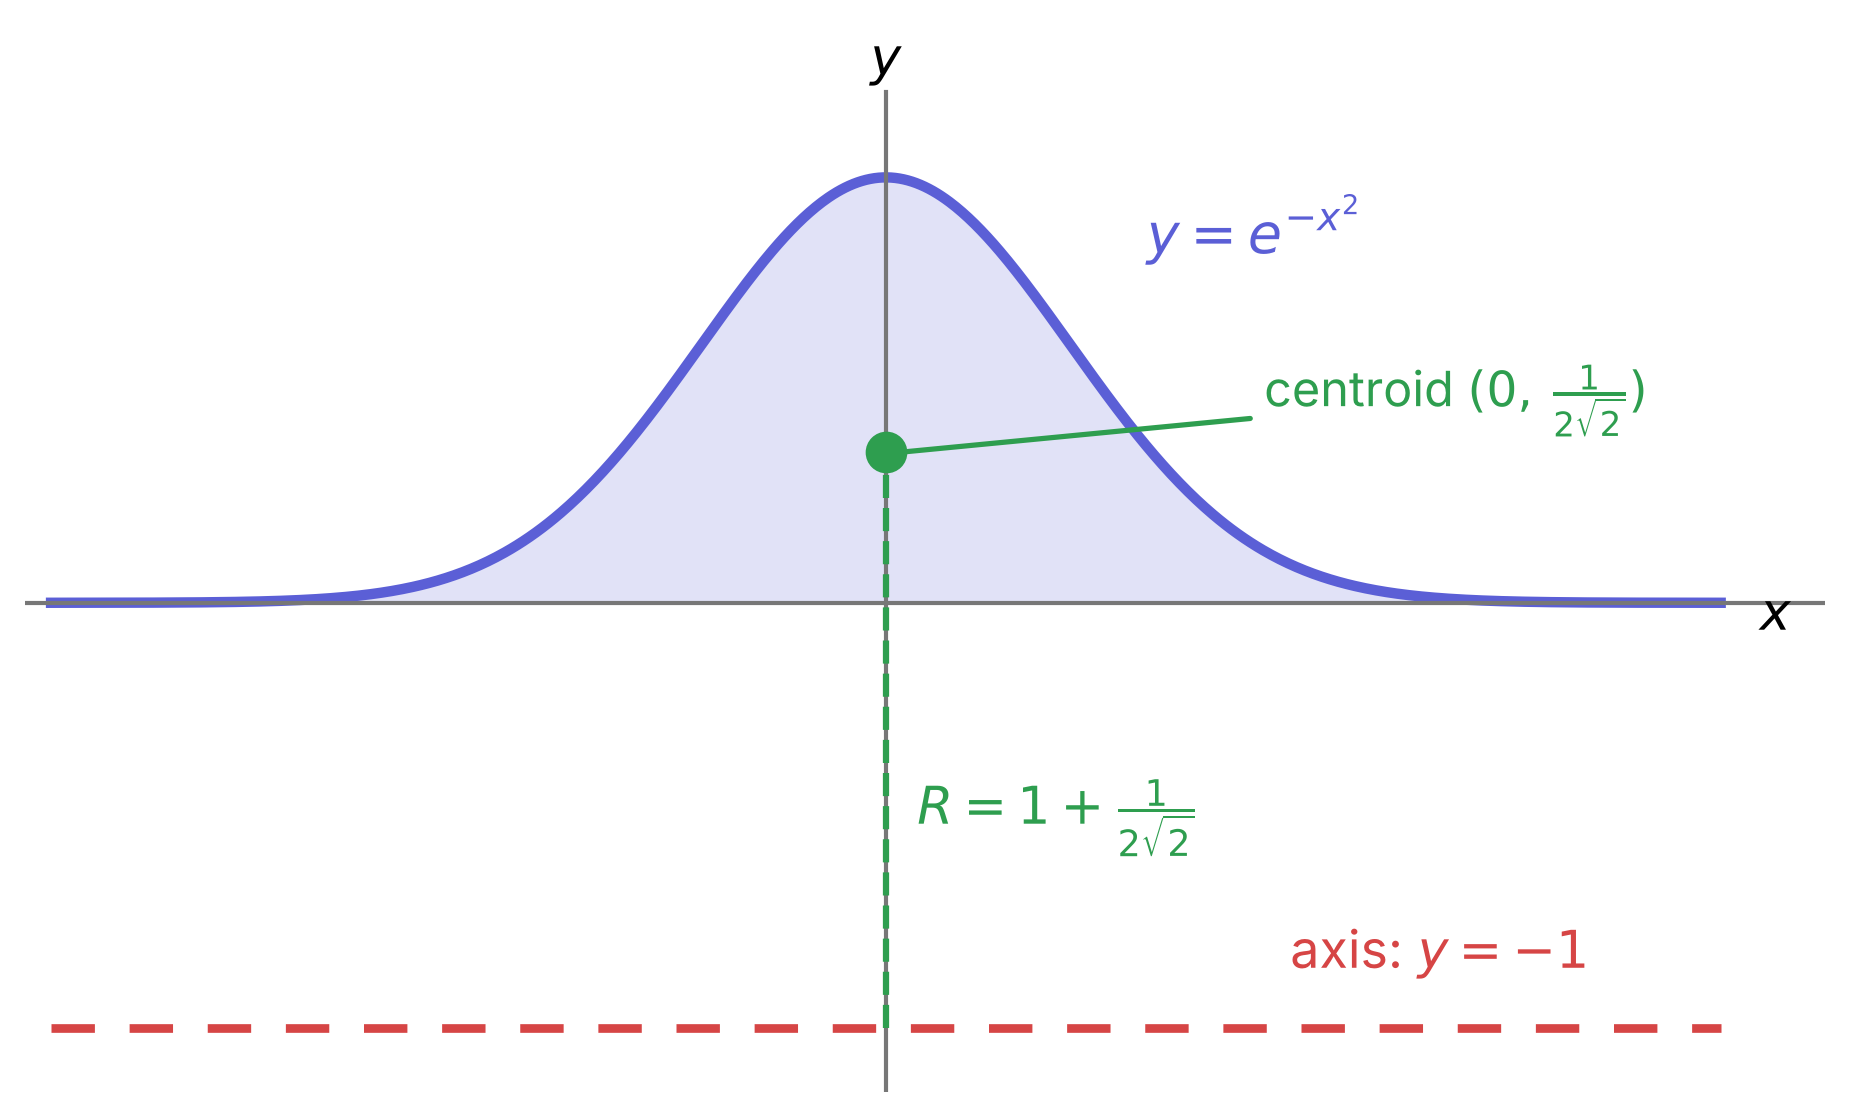
\includegraphics[width=0.75\textwidth]{figures/gauss_region.png}
\caption{Example~\ref{ex:gauss}. The region under $y=e^{-x^2}$ (shaded), its centroid $\bigl(0,\frac{1}{2\sqrt2}\bigr)$, and the axis of rotation $y=-1$ (red). The centroid is at distance $R=1+\frac{1}{2\sqrt2}$ from the axis, so it travels a circle of length $2\pi R$, and Pappus gives $V=\sqrt\pi\cdot2\pi R$.}
\label{fig:gaussregion}
\end{figure}

\begin{remark}
The rule needs the axis not to cut through $D$; otherwise parts of the solid are counted twice. Also, this is a statement about \emph{shapes}: a real rubber hose that you bend also changes its cross-section, so the physical volume can change.
\end{remark}

% ==================================================================
\section{One dimension up: when the cancellation fails}\label{sec:4d}
% ==================================================================

\begin{sidebox}{Box: Pappus in four dimensions (classical; Weyl 1939)}
In $\R^3$, a point at distance $\rho$ from the axis traces a \emph{circle}, of length $2\pi\rho$. In $\R^4$ there is room to spin a point so that it traces a whole \emph{2-sphere}, of area $4\pi\rho^2$. (Picture the usual sphere of radius $\rho$, sitting in a 3-dimensional slice of $\R^4$; the fourth coordinate is left alone.)

\medskip
\textbf{The experiment.} Take a disc of radius $r$ whose centre is at distance $R\ge r$ from the ``axis'' (the 2-plane that is kept fixed), and spin it this way. The centre traces a sphere of area $4\pi R^2$, so the naive Pappus guess is
\[
  V_{\text{guess}} = \pi r^2\cdot 4\pi R^2 = 4\pi^2R^2r^2 .
\]
\textbf{The true answer.} A small piece $\mathrm dA$ of the disc at offset $u$ from the centre (measured away from the axis) sweeps out volume $4\pi(R+u)^2\dd A$. So
\[
  V=\iint_{\text{disc}}4\pi(R+u)^2\dd A
   =4\pi\Bigl(R^2\!\iint \mathrm dA+2R\!\iint u\dd A+\iint u^2\dd A\Bigr)
   =4\pi\Bigl(\pi R^2r^2+0+\frac{\pi r^4}{4}\Bigr),
\]
that is,
\[
  \boxed{\,V=4\pi^2R^2r^2+\pi^2r^4\,}\qquad\text{versus}\qquad V_{\text{guess}}=4\pi^2R^2r^2 .
\]
The two are \emph{not} equal. (We used $\iint u^2\dd A=\int_0^{2\pi}\!\!\int_0^r \rho^2\cos^2\!\theta\,\rho\dd\rho\dd\theta=\pi r^4/4$.)

\medskip
\textbf{Why.} In $\R^3$ the weight $2\pi(R+u)$ is a \emph{linear} function of $u$, and the average of a linear function over a region is its value at the centroid. In $\R^4$ the weight $4\pi(R+u)^2$ is \emph{quadratic}: the outside gains more than the inside loses, and the leftover is $4\pi\iint u^2\dd A$. For example, with $R=r=1$ the true volume is $5\pi^2\approx 49.3$ against the guess $4\pi^2\approx 39.5$, which is $25\%$ more.

\medskip
\textbf{The deeper reason.} Why does a sweep along a \emph{curve} cancel perfectly, while a sweep along a \emph{sphere} leaves something over? The answer is curvature.

\emph{} Sweep a solid 3-ball of radius $r$ around a \emph{circle} of radius $R$ in $\R^4$. Each point travels a circle of length $2\pi(R+u)$, the weight is linear again, and $V=\tfrac43\pi r^3\cdot2\pi R=\tfrac83\pi^2Rr^3$ exactly. Sweeping along a curve always works; sweeping along a surface does not.

\emph{Intuition.} When you thicken a curved surface, the side facing outward is a slightly larger copy of the surface and the side facing inward is a slightly smaller one, just like the outer and inner fibres of the bent cylinder. For a curve the gain and loss are linear in the offset and cancel. For a surface they grow like the \emph{square} of the offset, and the leftover is controlled by how curved the surface is.

\emph{The formula.} Weyl's tube formula \cite{weyl,gray-tubes} makes this exact. If $M$ is a closed surface in $\R^4$ and $r$ is small, the set of points within distance $r$ of $M$ has volume
\[
  V(r)=\pi r^2\cdot\operatorname{Area}(M)+\frac{\pi}{4}\,r^4\int_M K\dd A ,
\]
where $K$ is the Gaussian curvature. The first term is the naive guess, a disc of area $\pi r^2$ times the area of $M$. The second term is the correction.

\emph{Check on our example.} For the sphere of radius $R$ we have $\operatorname{Area}=4\pi R^2$ and $K=1/R^2$ everywhere, so $\int_M K\dd A=4\pi$. The formula gives
\[
  V=\pi r^2\cdot 4\pi R^2+\frac{\pi}{4}r^4\cdot 4\pi=4\pi^2R^2r^2+\pi^2r^4,
\]
exactly the result of our direct computation above.

\emph{Why only the shape's topology matters.} The Gauss--Bonnet theorem says $\int_M K\dd A=2\pi\chi(M)$, where $\chi$ is the Euler characteristic ($\chi=2$ for a sphere, $\chi=0$ for a donut surface). So the leftover term is always $\tfrac{\pi^2}{2}\chi(M)\,r^4$: it depends only on how many holes $M$ has, not on its size or exact shape.

\emph{Back to the donut.} A torus surface is curved positively on its outer side and negatively on its inner side, and the two cancel: $\chi=0$. So sweeping a disc along a torus surface in $\R^4$ gives exactly ``area of disc $\times$ area of surface'', and the perfect cancellation of Section~2 returns. Curves have no intrinsic curvature at all, which is why Pappus is always exact for them.

All of this is classical (Weyl 1939; for sweeps along submanifolds see Domingo-Juan--Miquel \cite{domingo-miquel}; for curved spaces see Gray--Miquel \cite{gray-miquel} and Cho--Choi \cite{cho-choi}).
\end{sidebox}

% ==================================================================
\section{Slicing along a curve: centroid curves}\label{sec:centroid}
% ==================================================================

\subsection{A bent stack of coins}
Cavalieri's principle says that the volume of a solid is the integral of the areas of its parallel slices: a stack of coins has volume (area of a coin)$\times$(height of the stack). Now look at the doughnut again: it is a stack of discs, but the stack is \emph{bent} around a circle. Pappus's theorem says the volume is still (area of a disc)$\times$(length of the circle). Goodman and Goodman \cite{goodman} asked in 1969 how far this goes. Schmid \cite{schmid} recently gave a clean answer.

Take a solid $K$ in $\R^3$ and a curve $\gamma$ inside it, parametrised by arc length $s$, with unit tangent $T(s)$. At each point $\gamma(s)$ cut $K$ by the plane through $\gamma(s)$ perpendicular to $T(s)$. Let $A(s)$ be the area of the slice and $c(s)$ its centroid. Schmid proves (under a non-overlap assumption discussed in Section~\ref{sec:overlap})
\begin{equation}\label{eq:schmid}
  \vol(K)=\int A(s)\,\bigl(1-\bar u\,\kappa_n+\bar v\,\kappa_g\bigr)\dd s,
\end{equation}
where $\bar u,\bar v$ measure how far the slice's centroid $c(s)$ is from the curve, and $\kappa_n,\kappa_g$ measure how the curve bends. The correction factor is exactly the ``stretch/squash'' factor $1+x/R$ of Section~\ref{sec:cylinder}, averaged over the slice. If every slice is balanced on the curve, the correction disappears.

\begin{definition}
$\gamma$ is a \textbf{centroid curve} of $K$ if, for every $s$, the centroid of the slice through $\gamma(s)$ perpendicular to $\gamma$ is the point $\gamma(s)$ itself. Then
\[
  \vol(K)=\int A(s)\dd s \qquad\text{(a bent stack of coins).}
\]
\end{definition}

\noindent\textbf{Convention.} Throughout, ``the slice'' means the \emph{whole} intersection of $K$ with the plane. For convex bodies there is no other choice. For the torus this matters, and we come back to it in Section~\ref{sec:torus}.

\begin{example}[Easy centroid curves]\label{ex:easy}
\begin{enumerate}[nosep]
\item \emph{Ball, any diameter.} The slices are discs centred on the diameter. A line that misses the centre is \emph{not} a centroid curve: a slice perpendicular to it is a disc centred at the foot of the perpendicular from the centre of the ball, which is off the line.
\item \emph{Solid of revolution, its axis.} Every slice is a disc or an annulus centred on the axis. (So is any straight line along which $K$ is symmetric under rotation by $180^\circ$.)
\item \emph{A box, a line through the centre parallel to an edge.}
\end{enumerate}
\end{example}

These are all straight lines. Schmid showed that curved centroid curves exist near the boundary of any smooth convex body, and he left open three questions: \emph{Does such a curve extend all the way across the body? How many pass through a given point? What happens for non-convex bodies?} \cite{schmid}. Sections~\ref{sec:ellipsoid}--\ref{sec:torus} give partial answers.

\subsection{The key tool: the cut-off volume}
Fix a point $p$ inside $K$ and a unit vector $n$. Cut $K$ with the plane through $p$ perpendicular to $n$, and let
\[
  V(n,p)=\vol\{x\in K:\ (x-p)\cdot n\ge0\}
\]
be the volume of the part \emph{in front of} the plane. Write $A(n,p)$ for the area of the slice and $c(n,p)$ for its centroid. Two standard facts drive everything (see \cite[\S3]{schmid}):
\begin{enumerate}[label=(\roman*)]
\item \textbf{Pushing the knife.} Moving $p$ forward by a small distance $h$ in the direction $n$ removes a thin layer of volume $\approx A\,h$. So $\nabla_pV=-A\,n$.
\item \textbf{Tilting the knife.} Tilt the plane by a small angle $\delta$ about a line through $p$. A point of the slice at distance $\ell$ from the tilt line sweeps a wedge of thickness $\approx\delta\ell$, positive on one side and negative on the other. The total change is $\delta$ times the \emph{first moment} of the slice about the tilt line. In formulas: if $n=n(s)$ changes, then $\frac{\mathrm d}{\mathrm ds}V(n(s),p)=A\,(c-p)\cdot n'(s)$.
\end{enumerate}
The first moment about a line through $p$ is zero for every tilt line exactly when $p$ is the centroid. So:

\begin{center}
\fbox{\parbox{0.86\linewidth}{\centering $p$ is the centroid of the slice with normal $n$ $\iff$ $n$ is a critical point of $n\mapsto V(n,p)$ on the sphere of directions.}}
\end{center}

We call such $n$ a \textbf{barycentric direction} at $p$. A centroid curve is then simply a curve whose tangent is, at each of its points, a barycentric direction there. The subject becomes the study of a (possibly multi-valued) field of directions.

\begin{example}[Checking the tool on a ball]
Let $K$ be the unit ball and $\gamma(s)=(0,0,s)$. The cap above height $s$ has volume $f(s)=\pi\bigl(\tfrac23-s+\tfrac{s^3}{3}\bigr)$, and $f'(s)=-\pi(1-s^2)$, which is minus the area of the slice at height $s$, as fact~(i) predicts.
\end{example}

\paragraph{How many barycentric directions?} The following is standard. $V(\cdot,p)$ always has a minimum, so there is always at least one barycentric direction. The minimum value $v(p)=\min_nV(n,p)$ is called the \emph{depth} of $p$, and the ``main'' centroid curves follow the steepest-ascent lines of the depth (Schmid's Theorem~5 \cite{schmid} in other words). Since $V(-n,p)=\vol(K)-V(n,p)$, the minima and maxima come in pairs, and if all critical points are non-degenerate a Morse-theory count gives an \emph{odd} number $2m-1$ of barycentric directions (counting $\pm n$ once), where $m$ is the number of local minima. This needs $V(\cdot,p)$ to be smooth, which fails for polyhedra.

% ==================================================================
\section{Ellipsoids, completely}\label{sec:ellipsoid}
% ==================================================================

Let $E=\{x^2/a^2+y^2/b^2+z^2/c^2\le1\}$ with $a>b>c>0$, and write $M=\operatorname{diag}(1/a^2,1/b^2,1/c^2)$, so $E=\{x^TMx\le1\}$.

\begin{lemma}[Centre of a slice]\label{lem:B1}
The slice of $E$ by the plane $u\cdot x=t$ has centroid $\displaystyle\frac{t\,M^{-1}u}{u^TM^{-1}u}$.
\end{lemma}
\begin{proof}
$E$ is the image of the unit ball under the stretch $S=\operatorname{diag}(a,b,c)$. A slice of the ball is a disc centred at the point of the plane closest to the origin. A linear map sends a planar region's centroid to the centroid of its image, because it scales every area in that plane by the same factor. Applying $S$ to the disc centre and simplifying gives the formula.
\end{proof}

\noindent\emph{Two-dimensional sanity check.} For the ellipse $x^2/4+y^2\le1$ and the vertical line $x=1$, the formula gives centroid $(1,0)$: obvious by symmetry. For the line $x+y=1$ it gives $\frac{(4,1)}{5}=(0.8,0.2)$, the midpoint of the chord, which you can check by solving the quadratic.

\begin{theorem}[Exactly one slice is balanced at each point]\label{thm:B2}
For $p\ne0$ inside $E$, the only plane through $p$ whose slice has centroid $p$ is the plane with normal $Mp$, which is the plane tangent at $p$ to the smaller ellipsoid $x^TMx=p^TMp$. At $p=0$ every plane works.
\end{theorem}
\begin{proof}
By Lemma~\ref{lem:B1}, the centroid equals $p$ if and only if $p$ is parallel to $M^{-1}u$, that is, $u$ is parallel to $Mp$.
\end{proof}

\begin{theorem}[All centroid curves]\label{thm:B3}
Away from the centre, the centroid curves of $E$ are exactly the arcs of
\[
  (x,y,z)=\bigl(x_0\,\tau^{1/a^2},\;y_0\,\tau^{1/b^2},\;z_0\,\tau^{1/c^2}\bigr),\qquad 0<\tau\le\tau_{\max},
\]
the curves that cross every scaled copy of $E$ at right angles. Each runs from the centre (as $\tau\to0$) out to the boundary.
\end{theorem}
\begin{proof}
By Theorem~\ref{thm:B2} the tangent of a centroid curve must be parallel to $M\gamma$. Solve $\gamma'=M\gamma$, i.e.\ $x'=x/a^2$, $y'=y/b^2$, $z'=z/c^2$: this gives $x=x_0e^{\sigma/a^2}$, etc., and $\tau=e^{\sigma}$. The direction field is smooth away from $0$, so solutions are unique.
\end{proof}

Schmid found this formula for points with $x>0$ \cite[Prop.~7]{schmid}. What is new here is that the balanced plane is unique (Theorem~\ref{thm:B2}), which makes the list complete, and the following analysis of curves that go all the way across.

\begin{theorem}[Crossing curves]\label{thm:B4}
Let $\Gamma$ be a centroid curve joining two boundary points of $E$.
\begin{enumerate}[label=(\arabic*)]
\item $\Gamma$ passes through the centre exactly once. (Along a centroid curve that avoids $0$, the quantity $q=\gamma^TM\gamma$ is strictly monotone, so it cannot equal $1$ at both ends.)
\item $\Gamma$ is two curves from Theorem~\ref{thm:B3} glued at $0$. Each half arrives tangent to an axis: the $x$-axis if $x_0\ne0$, otherwise the $y$-axis if $y_0\ne0$, otherwise the $z$-axis. The glued curve is a ($C^1$) centroid curve exactly when both halves arrive along the same axis from opposite sides.
\item \textbf{Exact smoothness.} Over its arrival axis (say the $x$-axis) the curve is $y=\beta_\pm|x|^{a^2/b^2}$, $z=\gamma_\pm|x|^{a^2/c^2}$ for $\pm x>0$. Hence a generic crossing curve is $C^{k}$ with $k=\lfloor a^2/b^2\rfloor$, and no smoother. If $a^2<2b^2$, generic crossing curves have \emph{infinite curvature} at the centre.
\item $\displaystyle\int_\Gamma A\dd s=\vol(E)=\tfrac43\pi abc$, even though (as we will see) the slices overlap.
\end{enumerate}
\end{theorem}

\begin{example}[Infinite curvature]
Take $a^2/b^2=3/2$. Then generic crossing curves look like $y=\beta|x|^{3/2}$ near the centre. Since $y''=\tfrac34\beta|x|^{-1/2}\to\infty$, the curvature blows up at the centre. These curves are outside the $C^2$ setting of \cite{schmid}, but part~(4) still holds by Theorem~\ref{thm:A} below.
\end{example}

\begin{corollary}[Polynomial centroid curves]\label{cor:B5}
$E$ has a smooth crossing centroid curve that is not a straight line if and only if one of $a^2/b^2$, $a^2/c^2$, $b^2/c^2$ is an integer. In that case the curves $x_j=C\,x_k^{\,n}$ are polynomial.
\end{corollary}

\begin{example}[The $\sqrt2$-egg]\label{ex:egg}
Take $a=\sqrt2$, $b=1$ (and any $c<1$). Then $a^2/b^2=2$, and Theorem~\ref{thm:B3} gives $y=y_0\tau^{1}=y_0(x/x_0)^2$: \emph{every parabola $y=kx^2$ in the plane $z=0$ is a centroid curve} (Figure~\ref{fig:teaser}, left). You can check this in one line. At the point $p=(x,kx^2,0)$ the parabola's tangent is $(1,2kx,0)$, while Theorem~\ref{thm:B2} asks for the normal
\[
  Mp=\Bigl(\frac{x}{2},\,kx^2,\,0\Bigr)=\frac x2\,(1,\,2kx,\,0),
\]
which is parallel to the tangent. So every slice perpendicular to the parabola is balanced on it. Numerically, with $c=0.7$ and $k=0.6$, the largest distance between a slice's centroid and the parabola is $3\times10^{-31}$ and $\int A\dd s-\vol(E)\approx10^{-30}$, using exact slice areas and 30-digit arithmetic. Similarly, for $a:b:c=2:\sqrt2:1$ every curve $(x,\beta x^2,\gamma x^4)$ is a centroid curve.
\end{example}

\begin{sidebox}{In one sentence}
Take an egg whose long axis is $\sqrt2$ times its width, draw any parabola through its centre, and slice perpendicular to the parabola: the slices cut through each other, yet their areas add up exactly to the volume.
\end{sidebox}

% ==================================================================
\section{Pappus does not need the slices to be disjoint}\label{sec:overlap}
% ==================================================================

Look at the slices of the $\sqrt2$-egg along the parabola $y=0.6x^2$ (Figure~\ref{fig:cross}). Near the top of the picture they cross each other \emph{inside} the egg. Out of $1770$ pairs of sampled slices, $393$ pairs cross inside the body. Schmid's formula \eqref{eq:schmid} is proved under the assumption that the slices do not overlap, so it does not apply. Yet $\int A\dd s=\vol(E)$ holds to 30 digits. The overlap assumption is not needed.

\begin{figure}[h]
\centering
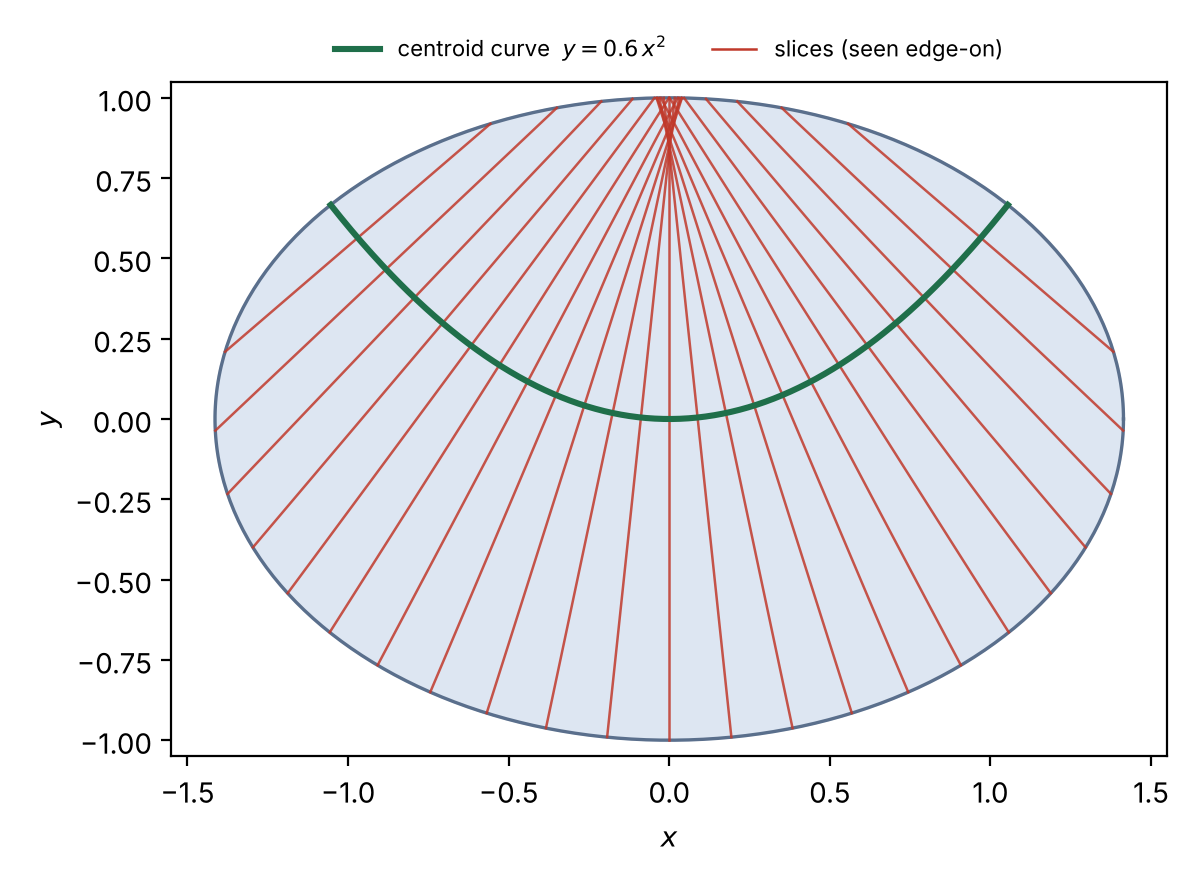
\includegraphics[width=0.62\textwidth]{figures/slices_cross.png}
\caption{The $\sqrt2$-egg ($a=\sqrt2$, $b=1$) seen from above, with the centroid curve $y=0.6x^2$ (green) and some of the slices perpendicular to it (red; each slice is a vertical plane, so it appears as a line). Slices from the two sides of the parabola cross near the top, inside the body. The areas still add up exactly to the volume (Theorem~\ref{thm:A}).}
\label{fig:cross}
\end{figure}

\begin{theorem}[Pappus without the no-overlap assumption]\label{thm:A}
Let $K$ be a convex body and $\gamma:[\alpha,\beta]\to K$ a curve parametrised by arc length, with unit tangent $T$ continuously differentiable except possibly at finitely many points. Let $f(s)=V(T(s),\gamma(s))$ be the volume in front of the slice at $\gamma(s)$. Then
\[
  f(\alpha)-f(\beta)=\int_\alpha^\beta A(s)\bigl(1-\bar u\kappa_n+\bar v\kappa_g\bigr)\dd s
\]
(as an improper integral if needed). If $\gamma$ is a centroid curve, the right-hand side is just $\int_\alpha^\beta A\dd s$. If moreover the first slice is tangent to $K$ with $K$ in front of it, and the last slice is tangent with $K$ behind it, then $\int_\alpha^\beta A\dd s=\vol(K)$.
\end{theorem}

\begin{proof}[Proof for centroid curves]
By the chain rule and the two facts of Section~\ref{sec:centroid},
\[
  f'(s)=\underbrace{\nabla_pV\cdot\gamma'(s)}_{\text{push}}+\underbrace{A\,(c-\gamma)\cdot T'(s)}_{\text{tilt}}
       =-A\,(T\cdot T)+A\,(c-\gamma)\cdot T' .
\]
For a centroid curve $c=\gamma$, so the tilt term vanishes and $f'(s)=-A(s)$. Integrate from $\alpha$ to $\beta$. At the first slice $f(\alpha)=\vol(K)$ (everything is in front) and at the last slice $f(\beta)=0$. At the finitely many points where $T$ is not differentiable, apply the fundamental theorem of calculus on the pieces in between and use that $f$ is continuous.
\end{proof}

For a general curve, writing $c-\gamma$ in Schmid's frame gives $(c-\gamma)\cdot T'=\bar u\kappa_n-\bar v\kappa_g$, which is the stated formula. Where $T'$ blows up (as in the infinite-curvature curves of Theorem~\ref{thm:B4}) the integral is improper, but it converges because the left side is finite.

The point of the proof is that we never cut the body into pieces. We only watch \emph{one number}, the volume in front of the knife, change as the knife moves. Overlapping slices are invisible to this argument. The derivative formulas behind it are in Schmid's \S3; as far as we know they have not been used before to remove the no-overlap assumption. This is a short observation, and we present it as such.

% ==================================================================
\section{Centrally symmetric convex bodies}\label{sec:symmetric}
% ==================================================================

Can a centroid curve that starts near the boundary always be continued across the body? For bodies with a centre of symmetry we can say yes, given one hypothesis.

\medskip
\noindent\textbf{Hypothesis (U).} For every $p\ne0$ inside $K$, the function $n\mapsto V(n,p)$ has a \emph{unique} minimiser $n(p)$.

\begin{theorem}[Global extension, assuming (U)]\label{thm:C}
Let $K$ be a convex body symmetric about $0$ and satisfying (U). Through every point $p\ne0$ there is a centroid curve that comes in from the boundary (its distance to the boundary tends to $0$) and reaches the centre after finite length. Gluing it to its mirror image $-\gamma$ gives a centroid curve through $p$ from boundary to boundary. Along the half from the boundary to $0$, $\int A\dd s=\vol(K)/2$.
\end{theorem}

\begin{proof}[Proof sketch, step by step]
\begin{enumerate}[label=(\roman*),nosep]
\item The unique minimiser $n(p)$ depends continuously on $p$, and the depth $v(p)=\min_nV(n,p)$ is differentiable with $\nabla v=-A\,n(p)$ (Danskin's theorem). Being a minimiser, $n(p)$ is a barycentric direction.
\item Solve $\gamma'=-n(\gamma)$. Along this curve $\frac{\mathrm d}{\mathrm ds}v(\gamma(s))=A>0$: the depth increases.
\item By symmetry every plane through $0$ cuts off exactly half, and $v<\vol/2$ everywhere else. On the region where $v\ge v(p)$, every slice contains a disc of a fixed radius $\rho>0$, so $A\ge\pi\rho^2$ there. Hence $v$ reaches $\vol/2$ within length $(\vol/2-v(p))/(\pi\rho^2)$, i.e.\ the curve reaches $0$.
\item Backwards in $s$ the depth decreases to $0$, which forces the curve to the boundary.
\item The reflected curve $-\gamma$ is also a centroid curve, and every plane through $0$ is barycentric. Finally $\int A\dd s=v(\text{end})-v(\text{start})=\vol/2-0$.\qedhere
\end{enumerate}
\end{proof}

\noindent\textbf{When does (U) hold?}
\begin{itemize}[nosep]
\item For ellipsoids it holds by Theorem~\ref{thm:B2}.
\item For the ``superball'' $x^4+y^4+z^4\le1$ it held at every point we sampled, and all 5 curves we traced reached the centre (numerical evidence only).
\item It \emph{fails} for the cube $[-1,1]^3$ on its central axes. At $p=(0,0,0.4)$, every plane that cuts the four vertical edges cuts off the same volume $4(1-0.4)=2.4$, so the minimiser is not unique.
\end{itemize}
\textbf{Open question.} Does (U) hold for every smooth, strictly convex, centrally symmetric body? It seems related to the smoothness of \emph{floating bodies} \cite{meyer-reisner}.

\begin{conjecture}[How curves arrive at the centre]
Generic centroid curves reach the centre tangent to a direction in which the central slice has \emph{locally smallest} area.
\end{conjecture}
This is true for ellipsoids: the central slice perpendicular to the long $x$-axis is the smallest one, and Theorem~\ref{thm:B4}(2) says generic curves arrive along the $x$-axis. For the superball the central slice is smallest perpendicular to the coordinate axes (area $3.708$, against $4.410$ and $4.443$ for the directions $(1,1,0)$ and $(1,1,1)$), and 3 of the 5 traced curves clearly arrive along an axis (numerical evidence only). A plausible proof route, through the ``intersection body'' of $K$, is sketched in the referee report in the code folder. The limiting behaviour near the centre is probably known in the floating-body literature, so we do not claim it.

% ==================================================================
\section{Corners: boxes and tetrahedra}\label{sec:corners}
% ==================================================================

\begin{proposition}[Corner lemma]
Near a vertex where exactly three edges meet, with edge vectors $e_1,e_2,e_3$, write $p=\lambda_1e_1+\lambda_2e_2+\lambda_3e_3$. The unique plane through $p$ that cuts off only that corner, with a triangle balanced at $p$, is the plane through the three points $3\lambda_ie_i$.
\end{proposition}
\begin{proof}
A triangle's centroid is the average of its three vertices, and $\tfrac13(3\lambda_1e_1+3\lambda_2e_2+3\lambda_3e_3)=p$.
\end{proof}

\begin{example}[Box corner: hyperbolas]
At a corner of a box (edges along the axes), the balanced plane through $p=(x,y,z)$ has normal $(1/x,1/y,1/z)$. A centroid curve satisfies $x'=1/x$, $y'=1/y$ (up to a common factor), so $\frac{\mathrm d}{\mathrm ds}(x^2-y^2)=2-2=0$. Hence the centroid curves near a corner are
\[
  x^2-y^2=C_1,\qquad x^2-z^2=C_2 .
\]
Only the diagonal $C_1=C_2=0$ reaches the vertex; all others meet a face at a right angle.
\end{example}

\paragraph{Tetrahedra.} Through the centroid of a tetrahedron there are at least 7 balanced planes: 4 parallel to the faces and 3 parallel to pairs of opposite edges (whose slices are parallelograms centred at the centroid). Our computer search finds exactly 7, but that is only numerical. Near a vertex, the corner lemma gives exactly one balanced plane among those that cut off that vertex alone; that it is the only balanced plane of any kind is so far only numerical (checked on three tetrahedra with two independent programs). Since the count changes from 1 to 7 \emph{inside a convex body}, there must be places where barycentric directions are born or die. Whether centroid curves get stuck there, as in the next section, is open.

% ==================================================================
\section{Back to the doughnut}\label{sec:torus}
% ==================================================================

We end where we started: the solid torus $T=\{(\sqrt{x^2+y^2}-2)^2+z^2\le1\}$, so $R=2$, $r=1$. It is the simplest solid that is not convex, and it gives three different answers to ``is this a centroid curve?''.

\paragraph{1. The core circle: yes for Pappus, no for whole slices.} Pappus slices the doughnut by \emph{local} discs around the core circle. Each disc is balanced on the circle, and the areas add up: $\pi r^2\cdot2\pi R=\vol(T)$. But the \emph{whole} plane perpendicular to the core circle at $(2,0,0)$ is the plane $y=0$, and it cuts the torus in \emph{two} discs, centred at $(2,0,0)$ and $(-2,0,0)$. Their common centroid is the centre of the hole, which is not on the circle. So with whole slices the core circle is not a centroid curve, and indeed $\int A\dd s=2\pi r^2\cdot2\pi R=2\vol(T)$: every disc is counted twice. For non-convex bodies, ``which slice?'' is a real question.

\paragraph{2. Straight lines: yes, even outside the body.} By symmetry, the vertical $z$-axis and every horizontal line through the centre are centroid curves for whole slices. The $z$-axis does not touch the torus at all, and yet $\int A\dd z=\vol(T)$ by Cavalieri. Centroid curves of non-convex bodies naturally live in the convex hull, not in the body.

\paragraph{3. Curves from the surface: they get stuck.} Now follow a centroid curve inward from the surface. By symmetry we can stay in the plane $y=0$ and only consider cutting planes whose normal $(\cos t,0,\sin t)$ lies in that plane. Then a direction $t$ is barycentric at $p$ exactly when a single number, the first moment $M_b(t)$ of the slice, is zero. For the torus this is a one-variable integral with an explicit integrand, which the computer can evaluate to about 12 digits. We found:

\begin{itemize}
\item \textbf{A fold (numerically).} In a thin lens around the equatorial plane ($|z|$ at most about $0.1$, for $0<x<1.6$) there are 3 barycentric directions. Outside it there is only 1. On the boundary of the lens two of the three merge and disappear, just as the two roots of $x^2=\varepsilon$ merge at $\varepsilon=0$ and disappear for $\varepsilon<0$. For example, at $(0.905,0,-0.098)$ the directions are at $40.8^\circ$, $46.3^\circ$ and $113.3^\circ$; at $(0.905,0,-0.102)$ only $113.1^\circ$ is left.
\item \textbf{The fold is real.} At $x=0.905$ this is proved with computer assistance; see Proposition~\ref{prop:fold} below.
\item \textbf{The curves die on the fold (numerically).} We traced 8 curves: 6 starting from points near the upper surface and 2 starting inside the lens. Each of them reaches the surface at one end, and at the other end runs into the fold and stops (red dots in Figure~\ref{fig:torus}). For example, the curve from $(1.15,0,0.5)$ ends at about $(0.91,0,-0.09)$, arriving at about $50^\circ$ to the horizontal while the fold there is nearly flat. Just beyond that point, the direction the curve needs no longer exists, so there is no smooth way to continue it. The only way on is to turn back along the other merging direction, which makes a cusp.
\end{itemize}

\begin{proposition}[The fold at $x=0.905$; computer-assisted]\label{prop:fold}
Consider cutting planes with normal $(\cos t,0,\sin t)$. At $p=(0.905,0,-0.098)$ at least three of them are balanced at $p$, while at $p=(0.905,0,-0.102)$ every balanced one has $105^\circ<t<120^\circ$. So two balanced directions merge and disappear between these two points.
\end{proposition}
\begin{proof}
Interval arithmetic (the Arb library \cite{arb}) returns an interval that is \emph{guaranteed} to contain the exact value of an integral, rounding errors included. At $p=(0.905,0,-0.098)$ it proves $M_b>0$ at $30^\circ$, $M_b<0$ at $43.5^\circ$, $M_b>0$ at $80^\circ$, $M_b<0$ at $130^\circ$, so by the intermediate value theorem there are at least 3 barycentric directions in the plane. At $p=(0.905,0,-0.102)$ it proves $M_b>0$ on all of $[0^\circ,105^\circ]$ and $M_b<0$ on all of $[120^\circ,180^\circ]$ (16{,}539 small intervals, about an hour on 4 cores), so the two directions near $41^\circ$ and $46^\circ$ have certainly disappeared.
\end{proof}

\begin{figure}[h]
\centering
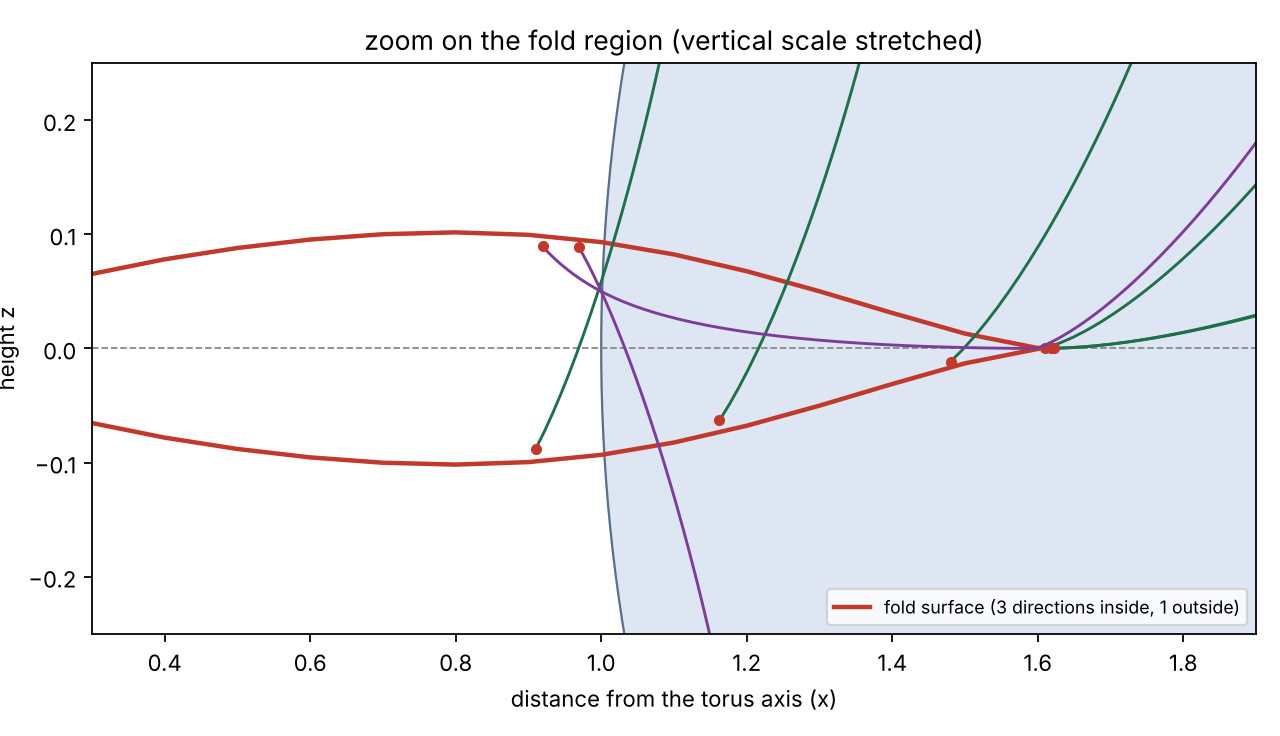
\includegraphics[width=0.8\textwidth]{figures/torus_fold_zoom.png}
\caption{Zoom on the fold region of Figure~\ref{fig:teaser} (right), with the vertical scale stretched. The red curves bound the lens with 3 barycentric directions. The green and purple centroid curves end on it (red dots).}
\label{fig:torus}
\end{figure}

So Schmid's question ``can a local centroid curve be extended through the whole body?'' has, for the solid torus, the answer \emph{no}: the curves we traced from the surface get stuck before reaching the other side. This is numerical evidence with a computer-assisted proof of the fold itself, not yet a theorem. Two things would make it one: a rigorous ODE solver showing that the traced curves really reach the fold, and certifying that no barycentric directions lie outside the plane $y=0$ (our 3-D search found none).

\paragraph{The full circle.} The same doughnut that Pappus used to show that bending a cylinder costs nothing turns out to be a place where bending \emph{does} cost something: if you insist on whole slices and start at the surface, the bent stack of coins cannot be completed.

% ==================================================================
\section{Summary}\label{sec:summary}
% ==================================================================

\begin{center}
\small
\begin{tabularx}{\linewidth}{>{\raggedright\arraybackslash}X l}
\toprule
\textbf{Statement} & \textbf{Status}\\
\midrule
Pappus's theorem, bent cylinder, 4D extra term $\pi^2r^4$ (Sections~\ref{sec:history}--\ref{sec:4d}) & known\\
Barycentric directions are critical points of the cut-off volume; odd count & known\\
Theorem~\ref{thm:A}: $\int A\dd s=\vol$ without the no-overlap assumption & proved\\
Ellipsoid: unique balanced plane, all centroid curves, crossing curves, exact smoothness, polynomial curves, $\sqrt2$-egg (Section~\ref{sec:ellipsoid}) & proved\\
Theorem~\ref{thm:C}: global extension for centrally symmetric bodies & proved, assuming (U)\\
(U) fails on the axes of a cube & proved\\
Arrival direction at the centre & conjecture (proved for ellipsoids)\\
Box-corner hyperbolas; $\ge7$ balanced planes at a tetrahedron's centroid & proved\\
Exactly 7 at the centroid; only 1 near a vertex & numerical\\
Torus: fold exists at $x=0.905$ & computer-assisted proof\\
Torus: traced centroid curves end on the fold & numerical\\
\bottomrule
\end{tabularx}
\end{center}

\paragraph{Novelty.} The ellipsoid results, Theorem~\ref{thm:C} and the torus fold do not appear in Schmid's paper, and we did not find them anywhere else; Theorem~\ref{thm:A} is a short observation. Our literature search was limited, so ``new'' here means ``not found by us''. The closest neighbouring work is Patáková, Tancer and Wagner \cite{ptw} on barycentric cuts of convex bodies.

\paragraph{Open problems.} (1) Prove the torus picture, or find a non-convex body with explicit slices (for example a prism over a non-convex planar region) where it can be done by hand. (2) Decide whether (U) holds for all smooth strictly convex symmetric bodies. (3) Prove the conjecture of Section~\ref{sec:symmetric}. (4) Do centroid curves get stuck inside a tetrahedron?

% ==================================================================
\section{How this work was done}\label{sec:howmade}
% ==================================================================

This paper was developed with AI assistance, and we want to be explicit about it. An AI check is good at catching algebra slips, missing hypotheses and numerical errors, but it is not a substitute for a mathematician reading the paper.

\bibliographystyle{plain}
\bibliography{refs}

% ==================================================================
\appendix
\section{The code, and what each script checks}\label{app:code}
% ==================================================================

All scripts are in the \texttt{code/} folder of this project. They need Python~3 with \texttt{numpy}, \texttt{scipy}, \texttt{sympy}, \texttt{mpmath} and \texttt{matplotlib}; the interval-arithmetic scripts also need \texttt{python-flint}. Install everything with
\begin{lstlisting}
pip install numpy scipy sympy mpmath matplotlib python-flint
\end{lstlisting}
Run each script from inside its own folder, e.g.\ \texttt{cd code/centroid\_curves} and then \texttt{python3 sympy\_checks.py}. The folder \texttt{code/centroid\_curves/} holds the original research code; \texttt{code/referee/} holds the independent check, written from scratch.

\subsection*{A.1 The few ideas the code uses}
\begin{itemize}
\item \textbf{Computing a slice.} Almost every script needs the area $A$ and centroid $c$ of the slice of a body by a plane. For a convex body (\texttt{smooth.py}) the program stands at $p$, looks in 400 directions within the plane, finds how far it can go before leaving the body (by bisection), and adds up thin triangles. For a box or tetrahedron (\texttt{box.py}) the slice is a polygon, computed exactly from where the plane meets the edges. For the torus (\texttt{torus\_exact.py}) the slice is cut into straight chords whose lengths have a formula, and the chords are added up by numerical integration.
\item \textbf{Finding barycentric directions.} The program asks: for which normal $n$ is the slice's centroid equal to $p$? It starts a root-finder from many initial guesses spread over the sphere and keeps every distinct answer (\texttt{dirs.py}, \texttt{box.bary\_dirs}).
\item \textbf{Tracing a centroid curve.} Take a small step $h$ in the current barycentric direction, find the barycentric direction at the new point that is closest to the old one, and repeat (\texttt{trace3d.py}, \texttt{torus\_exact.trace}). If there is no such direction nearby, the curve has hit a fold and the program stops.
\item \textbf{Interval arithmetic.} \texttt{referee/torus\_arb.py} redoes the torus integral with the Arb library, which returns an interval guaranteed to contain the exact value. A sign read off such an interval is a proof.
\end{itemize}

\subsection*{A.2 Script-by-script map}
{\footnotesize
\begin{xltabular}{\linewidth}{>{\ttfamily\raggedright\arraybackslash}p{3.4cm} >{\raggedright\arraybackslash}X >{\raggedright\arraybackslash}p{2.6cm} l}
\toprule
\normalfont\textbf{Script} & \textbf{What it does, in plain words} & \textbf{Checks} & \textbf{Time}\\
\midrule
\endhead
\multicolumn{4}{l}{\emph{code/centroid\_curves/ (original research code)}}\\
sympy\_checks.py & Symbolic algebra: the ellipsoid slice-centre formula; the box-corner triangle is balanced at $p$; $x^2-y^2$ stays constant along the corner curves. & Lemma~\ref{lem:B1}, corner lemma, box hyperbolas & seconds\\
ellipsoid\_check.py & At random points the plane with normal $Mp$ is balanced; along the parabola $y=0.6x^2$ every slice is balanced and the areas add up to the volume; counts slice pairs that cross inside (393). & Thm.~\ref{thm:B2}, Ex.~\ref{ex:egg}, Fig.~\ref{fig:cross} & $\sim$1 min\\
smooth.py & Library: area and centroid of a slice of a convex body $\{\varphi\le1\}$; defines ellipsoids and superballs. & used by others & --\\
dirs.py & Library: finds all barycentric directions at a point by root-finding from many starts. & used by others & --\\
trace3d.py & Library: traces a centroid curve in 3-D step by step. & used by others & --\\
superball\_run.py & Traces 5 centroid curves of $x^4+y^4+z^4\le1$ from near the boundary to the centre; saves \texttt{superball\_traces.json}. & Thm.~\ref{thm:C} numerics, conjecture & minutes\\
box.py & Library: exact polygon slices of a box (or any polyhedron given by its edges) and their barycentric directions. & used by \texttt{tetra\_check} & --\\
tetra\_check.py & Counts barycentric directions in a tetrahedron at the centroid and near a vertex. & Sec.~\ref{sec:corners}: 7 and 1 & minutes\\
raster.py & Library: slices of a non-convex body on a pixel grid (first rough exploration). & used by \texttt{torus\_trace} & --\\
planar\_reduce.py & Library: for bodies symmetric under $y\mapsto-y$, finds and follows directions inside the plane $y=0$. & used by \texttt{torus\_trace} & --\\
torus\_trace.py & First, rough tracing of torus centroid curves using the pixel grid; saves \texttt{torus\_traces.json}. Superseded by \texttt{torus\_exact.py}. & exploration only & minutes\\
torus\_exact.py & Library: high-precision torus slices (chords + adaptive integration, $\sim10^{-12}$), barycentric directions in the plane $y=0$, and curve tracing that stops at a fold. & Sec.~\ref{sec:torus} & --\\
torus\_run.py & Finds the fold height at 16 values of $x$ and traces curves from 6 points near the surface, in both directions (upwards they leave the body, downwards they end on the fold); saves \texttt{torus\_exact\_traces.json}. & Sec.~\ref{sec:torus}: fold, dead ends & $\sim$10 min\\
torus\_more.py & Traces the 2 curves that start inside the lens (purple), in both directions, and adds them to the same file. & Sec.~\ref{sec:torus} & minutes\\
make\_figs.py & Draws the torus and ellipsoid figures from the saved data into \texttt{figs/}. & Figs.~\ref{fig:teaser},~\ref{fig:torus} & seconds\\
\midrule
\multicolumn{4}{l}{\emph{code/referee/ (independent check, new code)}}\\
check\_ellipsoid.py & Re-derives the ellipsoid lemmas by a different method; tests Theorem~\ref{thm:A} on a curve that is \emph{not} a centroid curve (both sides agree to 21 digits); the $\sqrt2$-egg to 30 digits; recounts 393 of 1770. & Lemma~\ref{lem:B1}, Thms.~\ref{thm:B2}, \ref{thm:B3}, \ref{thm:A}, Ex.~\ref{ex:egg} & seconds\\
check\_polytopes.py & Fresh count for three tetrahedra (7 at the centroid, 1 near a vertex) and the cube counterexample to (U). & Sec.~\ref{sec:corners}, (U) & $\sim$10 min\\
check\_superball.py & Central-slice areas of the superball (3.708, 4.410, 4.443) and the limiting directions near the centre. & Conjecture, Sec.~\ref{sec:symmetric} & seconds\\
torus\_float.py & Torus slices derived independently (horizontal chords); reproduces the directions $40.8^\circ,46.3^\circ,113.3^\circ$ and their disappearance. & Sec.~\ref{sec:torus} & $\sim$1 min\\
torus\_arb.py & Library: the same integral in interval arithmetic (guaranteed error bounds). & used by \texttt{torus\_certify} & --\\
torus\_certify.py & Produces the certificates; output is in \texttt{torus\_certificates.txt}. & Sec.~\ref{sec:torus}: fold (computer-assisted proof) & $\sim$1 h\\
\midrule
\multicolumn{4}{l}{\emph{code/paper\_figs/}}\\
slices\_cross.py & Draws Figure~\ref{fig:cross} (overlapping slices of the $\sqrt2$-egg). & Fig.~\ref{fig:cross} & seconds\\
\bottomrule
\end{xltabular}}

\subsection*{A.3 Reproducing the main numbers}
\begin{lstlisting}
cd code/centroid_curves
python3 sympy_checks.py        # Lemma B1, corner lemma: prints True / 0
python3 ellipsoid_check.py     # sqrt(2)-egg, 393 crossing pairs
python3 torus_run.py           # fold + traces (about 10 minutes)
python3 torus_more.py
python3 make_figs.py           # figures into figs/

cd ../referee
python3 check_ellipsoid.py     # 30-digit checks
python3 torus_float.py         # 40.8, 46.3, 113.3 degrees
python3 torus_certify.py 4 "pts:0.905:-0.098:30,43.5,80,130"
python3 torus_certify.py 4 "cover:0.905:-0.102:0-105,120-180:0.01"   # ~1 hour
\end{lstlisting}
The last command appends to \texttt{torus\_certificates.txt}; the file shipped with the code already contains the results quoted in Section~\ref{sec:torus}.

\end{document}
